\section{Текущие результаты замеров}
Пока что замеры проводилиь только для конформаций сгенерированных в двумерном пространстве.
 
Как и ожидалось, неплотыне конформации оказались близки к одномерной модели изинга, в них не возникает намагниченность и нет фазового перехода. В свою очередь плотные графы близки к двумерной модели, и намагничиваются при низких температурах.

\begin{figure}[h]
	\centering
	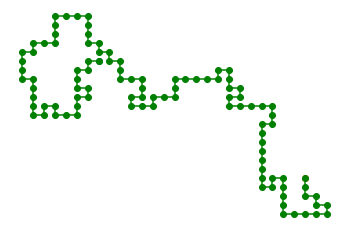
\includegraphics[width=0.45\textwidth]{../images/loose_conf.png}
	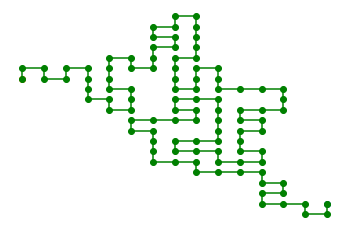
\includegraphics[width=0.45\textwidth]{../images/dense_conf.png} 
	%% add magnetization
	\caption{Пример неплотной и плотной конформации}
\end{figure}

В данный момент я занимаюсь нахождением точки фазового перехода в плотных графах.